\section{Arboles de decisión}
El arbol de desicion es un modelo grafico y analitico que se utiliza para tomar decisiones  basadas en diferentes condiciones. se representan en forma de un arbol donde: Los nodos internos representan preguntas o condiciones, las ramas representan posibles respuestas o decisiones  y las hojas representan una resultado o desicion final.

\section{Metodología}
El código del programa se descargo del documento AprendeMachineLearning y se ejecuto desde un google collab, el único problema causado por el código es que la funcion "sb.factorplot" había sido eliminada de versiones recientes de seaborn, asi que era necesario cambiar la funcion por otra igual, en este caso sb.catplot\\

La linea de código era: sb.factorplot('top',data=artists\_billboard,kind="count") \\
La nueva linea de código es sb.catplot(x='top', data=artists\_billboard, kind="count")

\section{Resultados}
El arbol de desicion resultante del codigo es el siguiente:
\begin{figure}[H]
    \centering
    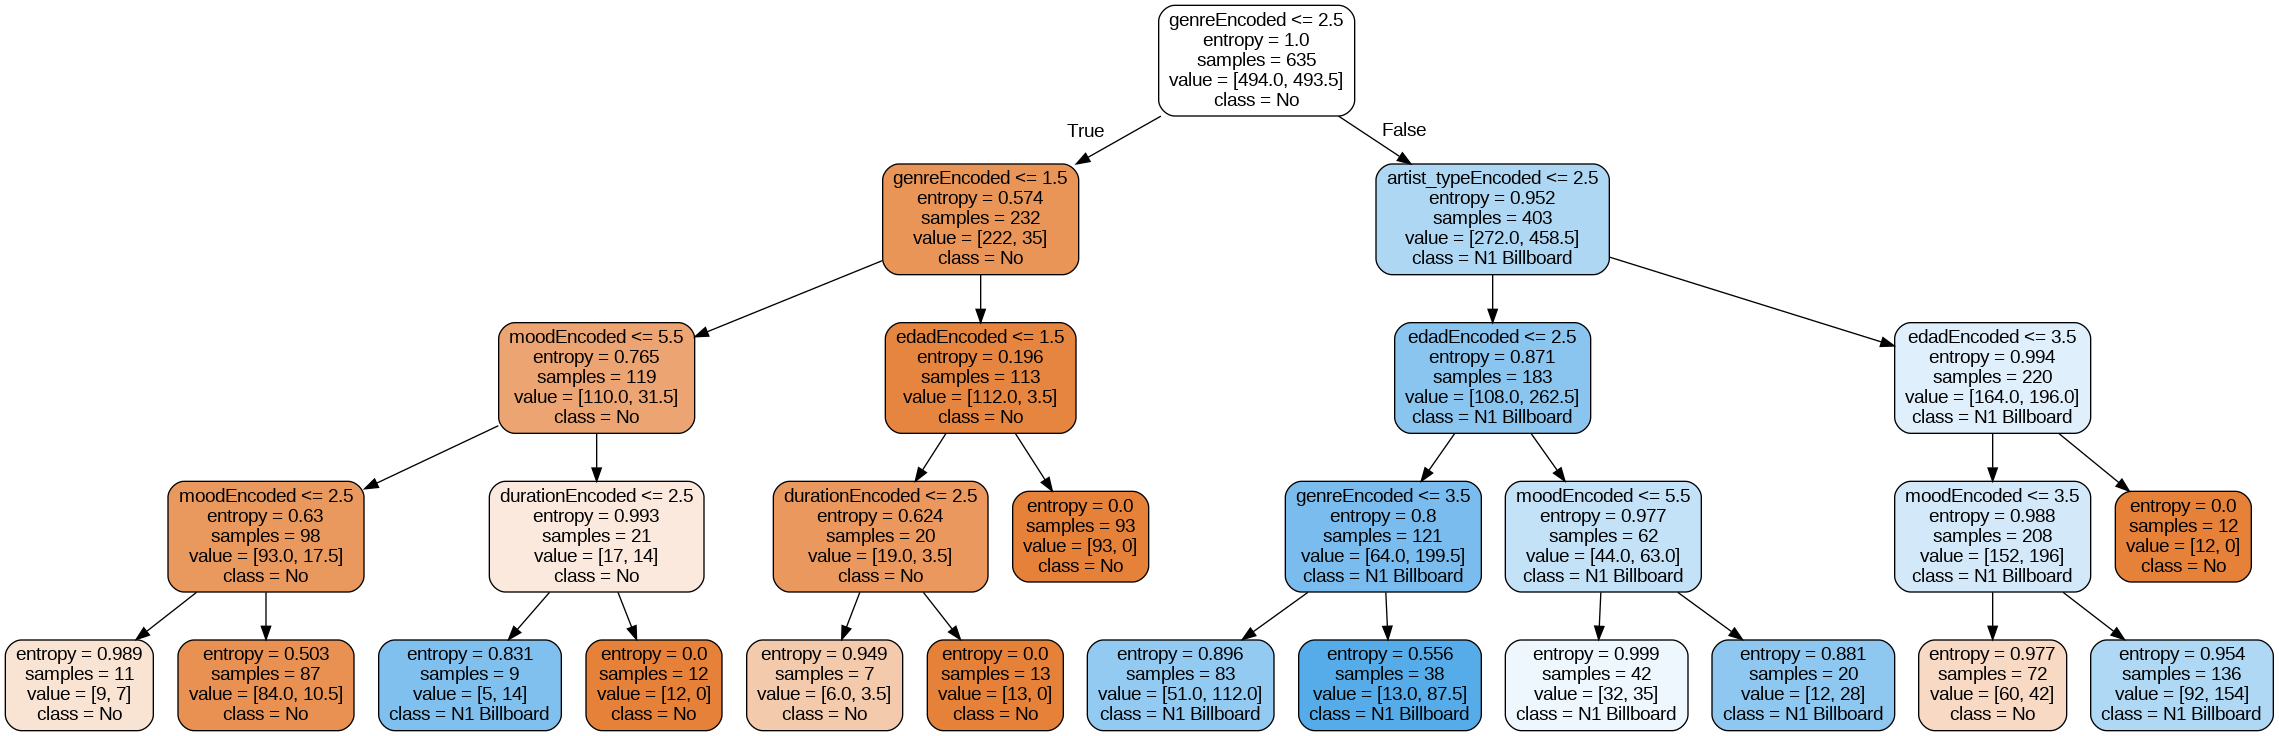
\includegraphics[width=1\linewidth]{resultados.png}
\end{figure}